%\documentclass{amsart}

\documentclass{article}
\usepackage[letterpaper,hmargin=15mm,vmargin=20mm]{geometry}
\usepackage[nosetup, colorlinks]{tony}
\usepackage{graphicx}

\usepackage{amsmath,amssymb}
\usepackage{siunitx}

\usepackage{mathpazo}
\usepackage{microtype}
\usepackage{multicol}

\usepackage{diagbox}

\usepackage{xcolor}
%\usepackage[printwatermark]{xwatermark}
%\newwatermark*[allpages,color=gray!50,angle=45,scale=3,xpos=0,ypos=0]{DRAFT}

\DeclareMathOperator{\sgn}{sgn}
\DeclareMathOperator{\NLL}{NLL}
\newcommand{\sind}[1]{^{(#1)}}

\title{6.867: Problem Set 3}
\date{November 10, 2016}

\begin{document}
\maketitle

\begin{multicols}{2}

% % % % % % % % % %
%    PROBLEM 1
% % % % % % % % % %

\section{Neural Networks}
\label{sec:nn}

\section{Convolutional Neural Networks}

% TODO connect from previous section

Empirically, deeper convolution networks work better.
To see why, we introduce the notion of \emph{receptive field}
of a node (a ``pixel" in a feature map):
the pixels from the original image that contribute information
to the node.

% What are the dimensions of the receptive field for a node in Z2?
For example,
suppose we have a convolutional network
with two successive convolutional layers,
with respective patch sizes $5\times 5$ and $3\times 3$.
Each layer has a single feature map (which we name $Z_1$ and $Z_2$).
Then the nodes in $Z_1$ each have $5\times 5$ receptive fields.
Nodes in $Z_2$ will have $(3 + 5 - 1)^2 = 7\times 7$ receptive fields.

% Thinking about your answer,
% why is it effective to build convolutional networks deeper
% (i.e. with more layers)?
In general,
nodes in deeper layers will have larger receptive fields,
so intuitively,
deeper convolutional networks should better detect large-scale structure.

% How many layers are there?
We tested an existing four-layer convolutional network implementation
on an image classification problem,
where given RGB images of 451 paintings by 11 artists
(all downsampled to $50\times 50$),
we would like to predict the artist that painted the given image.

% Are they all convolutional?
% If not, what structure do they have?
The first two layers are convolutional;
each produces 16 feature maps
with $5\times 5$ filters and stride $2$.
We zero-pad the feature maps prior to convolution
so that feature maps remain the same size ($50\times 50$).

Our last two layers are fully connected.
The third layer has 64 hidden units;
the final layer (our output) has 11 units,
corresponding to the 11 artists represented in our dataset.

% Which activation function is used on the hidden nodes?
The network applies a ReLU activation on all hidden nodes.

% What loss function is being used to train the network?
% How is the loss being minimized?
We train the network by minimizing softmax cross-entropy
through minibatch gradient descent,
with batches of 10 examples each.
Recall that average softmax cross-entropy is defined
for labeled examples $(x\sind{i}, y\sind{i})$
(where $y\sind{i}$ is a one-hot vector indicating the category of the example)
as
\begin{equation}
    H(y, \hat y) = \f{1}{n}\sum_{i=1}^n
                             \sum_{j=1}^k
                               y\sind{i}_j \log \hat y\sind{i}_j,
\end{equation}
where $\hat y\sind{i}$ is the prediction made by our network,
a vector of probabilities
produced by applying a softmax function
to the values on our output layer.
For instance, for our image classification problem,
$n$ is the number of images we are evaluating our network on,
and $k=11$ is the number of classification categories.

% What is the training accuracy for your network after training?
% What is the validation accuracy?
% What do these two numbers tell you about what your network is doing?
After 1500 training steps,
our convolutional network obtains perfect training accuracy,
but only $67\%$ validation accuracy,
strongly suggesting that our network is overfitting.

\subsection{Pooling}

% and choose different values for the pooling filter size and stride.
% After you applied max pooling, what happened to your results?
% How did the training accuracy vs. validation accuracy change?
We modified our network by adding max-pooling
after both convolutional layers.
We experimented with various pooling filter sizes (1 to 4)
and strides (1 to 4).
In all cases,
pooling modestly reduced training accuracy
(from around $100\%$ to $90\%$),
but did not improve validation accuracy noticeably.
Accuracy was typically $60\%$ to $70\%$.

Variations in validation accuracy
stemmed from the randomness inherent in our stochastic training scheme,
as variation in accuracy between runs with different hyperparameters
was comparable to the that between runs with the same hyperparameters.
% make less verbose?

% What does that tell you about the effect of max pooling on your network?
We conclude that max-pooling provides little improvement
to our convolutional network's accuracy.
We do note, however, that overfitting was reduced,
since training accuracy matched validation accuracy more closely.

\subsection{Regularization}

To combat the overfitting we saw earlier,
we tested various methods of regularization.
Unless otherwise stated,
in each section we \emph{only} vary the hyperparameter in question;
we leave the remaining hyperparameters (e.g. training steps, pooling) unchanged.

% Test each one individually,
% and discuss how it affects your results.

\subsubsection{Dropout}


We implemented dropout for the fully connected layer (the third layer).
We tested various values of dropout parameter~$p$,
the probability we do \emph{not} drop out a number.
For each $p$, we trained $n=10$ separate models;
we present the mean training and validation accuracies
with their respective standard errors here.
Training accuracies are quoted on the final minibatch of ten samples.
\begin{center}
    \begin{tabular}{c|cc}
        $p$ & Train $\pm 1 \sigma$ (\%) & Validation $\pm 1 \sigma$\\\hline
        0.6 &  $77.00 \pm 2.60$ & $62.18 \pm 0.81$ \\
        0.7 &  $75.00 \pm 3.42$ & $62.53 \pm 0.86$ \\
        0.8 &  $89.00 \pm 3.48$ & $65.52 \pm 1.24$ \\
        0.9 &  $94.00 \pm 2.21$ & $65.63 \pm 0.55$ \\
        1.0 & $100.00 \pm 0.00$ & $65.63 \pm 1.01$ \\
    \end{tabular}
\end{center}

% You should explore different values of dropout_prob
% to find one that works well.
While dropout reduces training accuracy significantly,
it only modestly affects validation accuracy.
So while dropout combats overfitting,
it doesn't improve our model's ability to generalize.

We also tested dropout together with pooling;
validation accuracies were slightly, but noticeably lower.


\subsubsection{Weight regularization}

As we did previously,  % TODO check that this is mentioned in previous section
we experimented with adding a regularization term
to our training loss.
In particular, we modify our softmax cross-entropy loss $\ell(w)$
to get a new loss
\begin{equation}
    \ell(w) + \lambda\sum_i \lVert w\sind{i} \rVert^2
\end{equation}
where we include an extra term:
the sum of the squared Frobenius norms of the weight matrices $w\sind{i}$,
weighted by a regularization parameter $\lambda$.

Again, we test each value of $\lambda$ ten times,
and present the mean accuracies (with associated standard errors) below.

\begin{center}
    \begin{tabular}{c|cc}
        $\lambda$ & Train $\pm 1 \sigma$ (\%) & Validation $\pm 1 \sigma$\\\hline
        0    & $100.00 \pm 0.00$ & $65.40 \pm 1.19$ \\
        0.01 & $100.00 \pm 0.00$ & $66.44 \pm 1.15$ \\
        0.03 & $100.00 \pm 0.00$ & $66.55 \pm 0.76$ \\
        0.1  & $100.00 \pm 0.00$ & $65.40 \pm 0.81$ \\
        0.3  &  $79.00 \pm 2.33$ & $52.64 \pm 1.36$ \\
      % 1.0  &  $50.00 \pm 0.00$ & $37.70 \pm 0.33$ \\
    \end{tabular}
\end{center}
Small values of $\lambda$ produced
statistically insignificant improvement in validation accuracies;
larger values saw significantly worse performance
in both training and validation accuracies.
Thus, weight regularization
is unlikely to be particularly helpful.


\subsubsection{Data augmentation}

We next enlarged our training dataset
with transformed versions of the original training samples
and trained on this augmented dataset.
This new dataset was four times as large as the original,
so we quadrupled the number of training steps
when working with the augmented training data.

We present our results as below.
As before, we repeat training ten times
and report means and standard errors.
\begin{center}
    \begin{tabular}{cc|cc}
        Augmented & Steps & Train $\pm 1 \sigma$ (\%) & Validation $\pm 1 \sigma$\\\hline
        No  & 1500 & $100.00 \pm 0.00$ & $65.98 \pm 1.03$ \\
%        No  & 6000 & $100.00 \pm 0.00$ & $66.21 \pm 0.86$ \\
        Yes & 6000 & $100.00 \pm 0.00$ & $62.30 \pm 0.61$
    \end{tabular}
\end{center}

Note that data augmentation actually lowered our validation accuracy.
Indeed, using the augmented data with 6000 steps
produced statistically significantly worse results
than using the original training set with 1500 steps
(Student's $t$-test, $p=0.0066$).


%    Finished training. Total time taken: 741.599348783493
%    Validation accuracies: [0.6091954,0.63218391,0.63218391,0.6091954,0.64367816,0.59770115,0.65517241,0.63218391,0.62068966,0.59770115]
%    Mean training accuracy: 100.00% +- 0.00%
%    Mean validation accuracy: 62.30% +- 0.61%
%    You ran command: conv.py --repeat 10 --augmented --training_steps 6001

%    Finished training. Total time taken: 591.5699789524078
%    Validation accuracies: [ 0.68965517,0.68965517,0.66666667,0.65517241,0.68965517,0.6091954,0.64367816,0.66666667,0.67816092,0.63218391]
%    Mean training accuracy: 100.00% +- 0.00%
%    Mean validation accuracy: 66.21% +- 0.86%
%    You ran command: conv.py --repeat 10 --training_steps 6001

%    Finished training. Total time taken: 151.98044800758362
%    Validation accuracies: [0.67816092,0.62068966,0.65517241,0.71264368,0.71264368,0.65517241,0.65517241,0.64367816,0.62068966,0.64367816]
%    Mean training accuracy: 100.00% +- 0.00%
%    Mean validation accuracy: 65.98% +- 1.03%
%    You ran command: conv.py --repeat 10 --training_steps 1501


\subsubsection{Early stopping}

Finally, we consider early stopping as a means of regularization.
We monitored the validation error
of our model each time we trained it;
we show a representative plot in Figure~\ref{fig:2-4-4-validation-acc}.

\begin{figure*}[t]
   \centering
   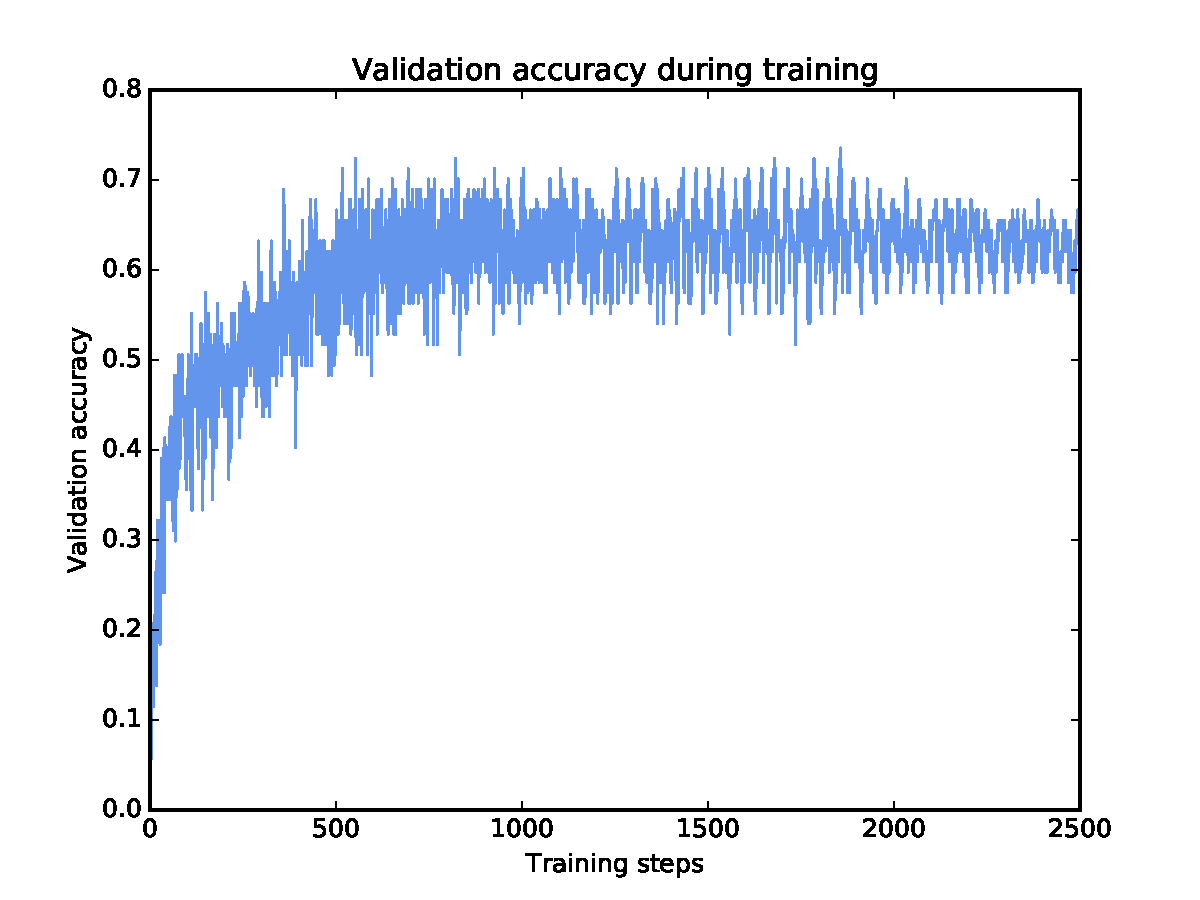
\includegraphics[width=4in]{img/2-4-4-validation-acc.pdf}
   \caption{Validation error of our convolutional network during training.}
   \label{fig:2-4-4-validation-acc}
\end{figure*}

After around 700 training steps,
validation accuracy fails to improve further.
We note, however, that validation accuracy does not \emph{decrease}
as we continue to train our model,
suggesting that overfitting (if it is occurring at all)
is not negatively impacting our results.



\subsection{Architecture variations}




\end{multicols}

\end{document}
